\chapter{Introduction}
\begin{itemize}
\item Vergeet niet verschillend opties te geven met bijvoorbeeld Mapping/localization.\\
\item Error analysis bij thrust profiles.\\
\item analytical results bij Inertias.\\
\end{itemize}



Mining technology has been improving for decades and mineshafts are dug up to three kilometers in depth. Consequently, these depths go along with grave dangers as shaft collaption, high temperatures and even exposure to toxic gasses. Especially the first one lead to mineworkers, that is why the mineshafts are up to regular inspection. At this moment, an inspector has to go inside the mines to big depths, to inspect walls for tears and cracks. Simultaniously, could the mine be under great pressure and could be collapsing any time. A way must be found to deduct this danger to a human being.\\

Unmanned Aerial Vehicle (UAV) usage application may be possible for use as a substitution for mining inspections. The application of multirotor copters is widely increasing. Drones have been used for numerous reason already, i.e. UAV Aerial Imaging, surveying, mapping, and making video footages from almost impossible angles. Also UAV inspection is an uprising application as well. Drones can substitude human kind with thereby preventing humans in encountering lifethreatning danger.\\

To accomplish the usage of drones inside mines, the drone has to be able to perform a mission. Fly a drone into a specific area, taking a picture and fly out again. It basically has to be deployed autonomously in a constrained environment (tight spaces, no GPS) performing a mapping and reconnaissance mission and bring back the data. the following issues need to be resolved for that to function: Firstly, sensor integration on the platform, such that obstacle avoidance can be done, secondly, a localization mechanism has to be found, and lastly, autonomous control of the platform. \\

This report is divided in different chapters ......\\





















































%The system for assignment 1 is presented in figure \ref{1} and \ref{1t1}
%\begin{figure}[H]
%\centering
%\includegraphics[width=\textwidth]{1.png}
%\caption{Pinned-sliding beam system}
%\label{1}
%\end{figure}
%\begin{table}[H]
%\centering
%\caption{Beam properties}
%\label{1t1}
%\begin{tabular}{|l|l|l|}
%\hline
%Length l				& 1									& m	\\ \hline
%Young's Modulus E:		& 2.1$\cdot$10\textsuperscript{11}	& N/m\textsuperscript{2} \\ \hline
%Cross section A:		& 10\textsuperscript{-4}			& m\textsuperscript{2}\\ \hline
%Mass density $\rho$:	& 7850								& kg/m\textsuperscript{3}\\ \hline
%Second moment of are I:	& 1\textsuperscript{-8}/12			& m\textsuperscript{4} \\ \hline
%\end{tabular}
%\end{table}
%
%\section{Analytical Solution}
%A beam with a pinned boundary condition on one end and a sliding boundary condition on the other end (as seen in Figure \ref{1}) is similar to a pinned-pinned beam. If the pinned-pinned beam is split through the middle, and a sliding boundary condition is applied, the beam system from Figure \ref{1} is found. Since the sliding boundary condition does not allow the beam to rotate, only the eigenfrequencies of the pinned-pinned beam where the center of the beam is horizontal are considered. This means only the odd $\lambda_i$ of the pinned-pinned beam are used in the pinned-sliding situation. Because the pinned-pinned beam is split into two parts, $\lambda$ needs to be divided by two as well $\lambda_{Ok}$ can be calculated using Equation \ref{eq:111}.
%
%\begin{equation}
%\lambda_{k}=(2\cdot k-1)\frac{\pi}{2}
%\label{eq:111}
%\end{equation}
%
%Using $\lambda_{k}$ and the beam properties from Table \ref{1t1}, the natural frequency $f_{k}$ can be calculated using Equation \ref{eq:112}.
%
%\begin{equation}
%f_k=\frac{\lambda_k^2}{2\pi L^2}\left( \frac{EI}{m} \right)^{1/2}
%\label{eq:112}
%\end{equation}
%\newpage
%The eventual eigenfrequencies can be found in Table \ref{11t1}.
%
%\begin{table}[H]
%\centering
%\caption{Eigenfrequencies of a pinned-sliding beam system}
%\label{11t1}
%\begin{tabular}{|l|l|l|l|}
%\hline
%Eigenmode	& $\lambda_{Ok}$	[-]	& $f_{Ok}$ [Hz]	& $\omega_{Ok}$ [rad/s] \\ \hline
%1	& $\frac{1}{2}\pi$ 	&	5.8633  &	36.840   \\ \hline
%2	& $\frac{3}{2}\pi$ 	&	52.770	&   331.56   \\ \hline
%3	& $\frac{5}{2}\pi$ 	&   146.58	&	921.01	\\ \hline
%4	& $\frac{7}{2}\pi$ 	&   287.30 	&   1805.2    \\ \hline
%5	& $\frac{9}{2}\pi$ 	&   474.93  &   2984.1    \\ \hline
%6	& $\frac{11}{2}\pi$	&   709.46	&   4457.7    \\   \hline      
%\end{tabular}
%\end{table}
%
%The equation for the mode shape $\tilde{y}_k$ remains the same, since only $\lambda_{Ok}$ has changed, has resulted in Equation \ref{eq:113}.
%
%\begin{equation}
%\tilde{y}_k=\textsf{sin}\left( \lambda_{Ok} \frac{x}{L} \right)
%\label{eq:113}
%\end{equation}
%
%The first six mode shapes are calculated with Equation \ref{eq:113} and plotted in Figure \ref{111}.
%
%\begin{figure}[H]
%\centering
%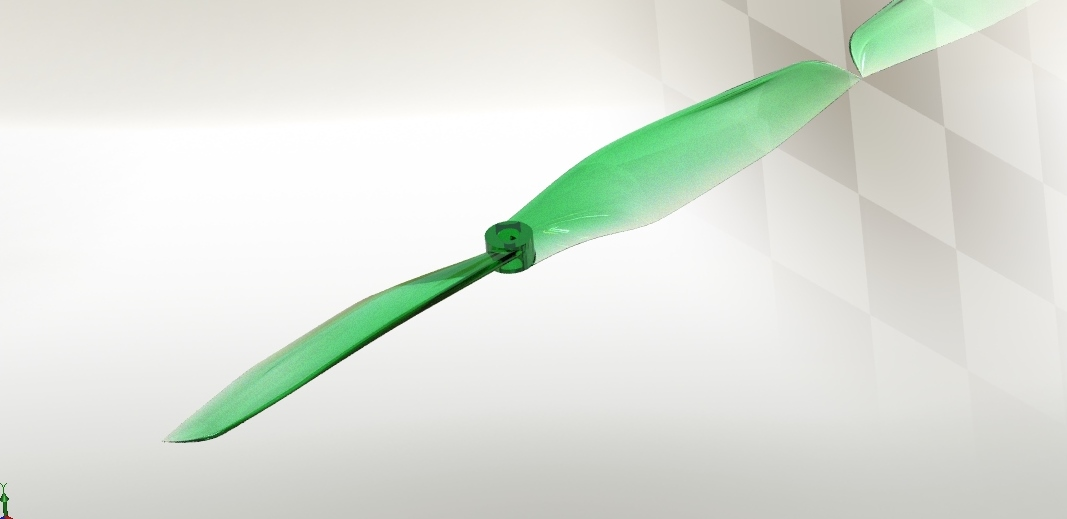
\includegraphics[width=\textwidth]{111.eps}
%\caption{Mode shapes of a pinned-sliding beam system}
%\label{111}
%\end{figure}
%
%
%\section{Finite Element Model Eigenfrequencies}
%Now, a finite element model is used to calculate the eigenfrequencies of the undamped pinned-sliding beam system.
%\begin{enumerate}[a)]
%\item  First, the mass en sitffness matrix of each beam element is constructed using Equation \ref{eq:12a1} and \ref{eq:12a2}.
%
%\begin{equation}
%K^e=\frac{EI}{l^3}\left[\begin{matrix}
%12	& 6l	& -12	& 6l	\\
%	& 4l^2	& -6l	& 2l^2	\\
%	&		& 12	& -6l	\\
%sym	&		&		& 4l^2
%\end{matrix}\right]
%\label{eq:12a1}
%\end{equation}
%
%\begin{equation}
%M^e=\frac{\rho Al}{420}\left[\begin{matrix}
%156	& 22l	& 54	& -13l	\\
%	& 4l^2	& 13l	& -3l^2	\\
%	&		& 156	& -22l	\\
%sym	&		&		& 4l^2
%\end{matrix}\right]
%\label{eq:12a2}
%\end{equation}
%
%These element matrices are combined into a global mass and stiffness matrix, with a size of (M+1)$\times$(M+1), where M is the amount of elements into which the beam is split up. Since the first node of the finite element model of the beam has a pinned constraint, the translation is 0. The last node of the beam has a sliding constraint, resulting in a rotation of 0. These two boundary conditions are applied to the global mass and stiffness matrices by removing the first and last column and row of each matrix. The eigenvalues of the pinned-sliding beam system can now be determined by solving the linear eigenvalue problem described in Equation \ref{eq:12a3}.
%
%\begin{equation}
%(\gamma_kM+K)u_{Ok}=0, \textsf{with } \gamma_k=\lambda^2_k=-\omega^2_{Ok}
%\label{eq:12a3}
%\end{equation}
%
%The first six eigenfrequencies of the pinned-sliding beam system are calculated with the help of the MATLAB function 'eig'. The results can be found in Table \ref{12at1}. The frequencies calculated with the finite element model are equal to the analytically calculated frequencies, although the finite element model has some small inaccuracies if a low amount of elements is used. The simulation time is increased rapidly when more elements are used. If 10000 elements are simulated, an out-of-memory error occurs.
%
%\begin{table}[H]
%\centering
%\caption{The six lowest eigenfrequencies of the pinned-sliding beam system }
%\label{12at1}
%\begin{tabular}{|l|l|l|l|}
%\hline
%Amount of elements [-] & 10 	& 100 		& 1000 \\ \hline
%cpu-time 'eig' [s]           & 0.0012  	& 0.0084    	& 2.319     \\ \hline
%Eigenfrequency 1 [Hz]  & 5.8633 & 5.8633    & 5.8435     \\ \hline
%Eigenfrequency 2 [Hz]  & 52.772 & 52.770    & 52.768     \\ \hline
%Eigenfrequency 3 [Hz]  & 146.62 & 146.58    & 146.58     \\ \hline
%Eigenfrequency 4 [Hz]  & 287.58 & 287.30    & 287.30      \\ \hline
%Eigenfrequency 5 [Hz]  & 476.18 & 474.93    & 474.93     \\ \hline
%Eigenfrequency 6 [Hz]  & 713.50 & 709.46	& 709.46     \\ \hline
%\end{tabular}
%\end{table}
%\newpage
%\item The lowest six eigenvalues are also calculated with MATLAB function 'eigs'. The results can be found in Table \ref{12bt1}.
%
%\begin{table}[H]
%\centering
%\caption{The six lowest eigenfrequencies of the pinned-sliding beam system}
%\label{12bt1}
%\begin{tabular}{|l|l|l|l|l|l|}
%\hline
%Amount of elements [-] & 10 	& 100 		& 1000		& 10000		& 100000	\\ \hline
%cpu-time 'eigs' [s]           & 0.0936	& 0.0937 	& 0.108    & 0.212		& 1.562	\\ \hline
%Eigenfrequency 1 [Hz]  & 5.8633 & 5.8633   	& 5.8633    & 5.8801	& 5.8633	\\ \hline
%Eigenfrequency 2 [Hz]  & 52.772	& 52.770   	& 52.770    & 52.771	& 52.770	\\ \hline
%Eigenfrequency 3 [Hz]  & 146.62 & 146.58   	& 146.58    & 146.58	& 146.58	\\ \hline
%Eigenfrequency 4 [Hz]  & 287.58 & 287.30   	& 287.30    & 287.30 	& 287.30	\\ \hline
%Eigenfrequency 5 [Hz]  & 476.18 & 474.93   	& 474.93    & 474.93	& 474.93	\\ \hline
%Eigenfrequency 6 [Hz]  & 713.50 & 709.46   	& 709.46    & 709.46	& 706.46	\\ \hline
%\end{tabular}
%\end{table}
%
%The difference between 'eig' and 'eigs' is that 'eig' calculates the same amount of eigenfrequencies as the length of the global mass or stiffness matrix after the application of boundary conditions, so in this case 'eig' calculates 2M-2 eigenfrequencies. With 'eigs', only the six lowest eigenfrequencies are calculated, resulting in a lower computation time for large amounts of elements. 
%
%\item  When the analytical results from Table \ref{11t1}, are compared with the simulation results from Table \ref{12at1} and \ref{12bt1}, the accuracy of the simulation models seems to improve. The models are already accurate for a low amount of elements (e.g. 10). 2 values are not as expected: when calculating the first eigenfrequency with 'eig', this frequency has a larger error at 1000 elements then when 10 or 100 elements are used. The same happens when the first two eigenfrequencies are calculated with 'eigs'. This is probably due to a numerical error, caused by MATLAB.\\
%
%The computation time of 'eigs' is significantly lower, since only the six lowest eigenfrequencies are calculated. For example, at 1000 elements, 'eig' needs 2.32 seconds to calculate the six lowest eigenfrequencies, where 'eigs' needs only   0.11 seconds.
%\end{enumerate}
%
%\section{Frequency Response Functions}
%In this part of the assignment the frequency response function of several damped and undamped configurations will be  calculated and displayed. Only the excitation and response at the last node  will be considered, over a frequency range of 0.2 to 500 Hz. All calculations use the finite element model as developed in Exercise 1.2
%\begin{enumerate}[a)]
%\item Three different methods have been used to calculate the frequency response function of the last node of the pinned-sliding beam system. First of all, the inverse of the dynamic stiffness matrix is calculated for frequencies between 0.2 and 200 Hz. The dynamic stiffness matrix can be calculated with Equation \ref{eq:13a1}. Since no damping is applied yet, $B$ is equal to 0. The inverse of the dynamic stiffness matrix corresponds with the transfer function matrix.
%\begin{equation}
%K_{dyn}=-4\pi^2f^2M+2\pi jfB+K
%\label{eq:13a1}.
%\end{equation}
%Since only the the transversal displacement of the last node is needed, the last diagonal element of this matrix is plotted for each frequency, in Figure \ref{13a1}. Calculating these values takes 3.02 seconds. The resonances and anti-resonances can clearly be seen in the magnitude plot. The six eigenfrequencies visible in the figure correspond with the eigenfrequencies calculated in Table \ref{11t1}. The response switches from a positive real number to a negative real number several times, resulting in phase changes of 180 degrees.
%\begin{figure}[H]
%\centering
%\includegraphics[width=\textwidth]{13a1.eps}
%\caption{FRF calculated with the inverse of the dynamic stiffness matrix}
%\label{13a1}
%\end{figure}
%The second method used to calculate the transfer function matrix is with Equation \ref{eq:13a2}. A modal superposition of the first six eigenmodes is used, resulting in a computation time of 1.84 seconds. The FRF of the last node is again found by taking the last diagonal element of each transfer function matrix.
%\begin{equation}
%H(\omega)=\sum_{k=1}^6 \left[ \frac{u_{Ok}u_{Ok}^T}{m_k(\omega_{Ok}^2-\omega^2} \right]
%\label{eq:13a2}
%\end{equation}
%In Figure \ref{13a2} the FRF calculated with the dynamic stiffness matrix is compared with the FRF calculated with Equation \ref{eq:13a2}. At low frequencies, the two graphs overlap, but at higher frequencies, some small inaccuracies can be seen due to the modal superposition that is used.
%\begin{figure}[H]
%\centering
%\includegraphics[width=\textwidth]{13a2.eps}
%\caption{FRF calculated with Equation \ref{eq:13a2}}
%\label{13a2}
%\end{figure}
%\newpage
%The third way used to calculate the transfer function matrix is with Equation \ref{eq:13a3}, which is similar to Equation \ref{eq:13a2}, but now all eigenmodes are used to calculate the FRF of the last node. The computation time for this method is 61.0 seconds, a lot more than the two previous methods.
%\begin{equation}
%H(\omega)=\sum_{k=1}^n \left[ \frac{u_{Ok}u_{Ok}^T}{m_k(\omega_{Ok}^2-\omega^2} \right]
%\label{eq:13a3}
%\end{equation}
%In Figure \ref{13a3} the FRF calculated with Equation \ref{eq:13a3} is compared with the FRF calcuated with the dynamic stiffness matrix. The dynamic stiffness matrix FRF and the FRF from Equation \ref{eq:13a3} seem to have exactly the same shape. The dynamic stiffness matrix FRF has a relatively low calculation time and a significantly high accuracy. In the other questions of this exercise the modal superposition calculation will be used to determine all FRF's. 
%\begin{figure}[H]
%\centering
%\includegraphics[width=\textwidth]{13a3.eps}
%\caption{FRF calculated with Equation \ref{eq:13a3}}
%\label{13a3}
%\end{figure}
%\newpage
%\item Now, damping is added to the system, with a damping coefficient $\xi_k$ of 0.02 for each mode. The transfer function matrix is now calculated with Equation \ref{eq:13a4}, where an extra term for damping is added.
%\begin{equation}
%H(\omega)=\sum_{k=1}^6 \left[ \frac{u_{Ok}u_{Ok}^T}{m_k(\omega_{Ok}^2-\omega^2+2j\xi_k\omega\omega_{Ok})} \right]
%\label{eq:13a4}
%\end{equation}
%The FRF is again the last diagonal value of the transfer function matrix calculated in Equation \ref{eq:13a4}. This FRF is plotted in Figure \ref{13b1}. Comparing with Figure \ref{13a1}, the peaks of the function are lower and more rounded, which is a direct result of the added damping. Furthermore, the transition between the positive and negative values is more smooth, which is a result of the complex component added by the damping. The eigenfrequencies can still be seen very clearly in the magnitude plot.
%\begin{figure}[H]
%\centering
%\includegraphics[width=\textwidth]{13b1.eps}
%\caption{FRF with proportional damping, $\xi$=0.02}
%\label{13b1}
%\end{figure}
%The first six eigenvalues with positive complex values are given in Table \ref{13bt1}. The complex part of the eigenvalues is equal to the eigenfrequencies of the undamped system (in rad/s), as can seen in Table \ref{12at1}.
%\begin{table}[H]
%\centering
%\caption{Eigenvalues of the proportionally damped system}
%\label{13bt1}
%\begin{tabular}{|l|l|}
%\hline
%Eigenmode & Eigenvalue [-]  \\ \hline
%1         & -0.737+36.8i \\ \hline
%2         & -6.63+332i   \\ \hline
%3         & -18.4+921i   \\ \hline
%4         & -36.1+1805i  \\ \hline
%5         & -59.7+2984i  \\ \hline
%6         & -89.2+4458i  \\ \hline
%\end{tabular}
%\end{table}
%\newpage
%\item The Rayleigh damping model uses Equation \ref{eq:13c1} to assemble the damping matrix $B$. 
%\begin{equation}
%B=\alpha M+\beta K
%\label{eq:13c1}
%\end{equation}
%If this expression is mass normalized, it can be written as in Equation \ref{eq:13c2}.
%\begin{equation}
%U_O^TBU_O=U_O^T\left(\alpha M+\beta K\right) U_O=\alpha U_O^TMU_O+\beta U_O^TKU_O=B^*=\alpha I+\beta \Omega_O^2
%\label{eq:13c2}
%\end{equation}
%The diagonals from these matrices are equal as well, which results in Equation \ref{eq:13c3}.
%\begin{equation}
%2\xi_k\omega_{Ok}=\alpha+\beta \omega_{Ok}^2
%\label{eq:13c3}
%\end{equation}
%This can be rewritten to Equation \ref{eq:13c4} to find the final expression for $\xi_k$.
%\begin{equation}
%\xi_k=\frac{1}{2}\left(\frac{\alpha}{\omega_{Ok}}+\beta \omega_{Ok}\right)
%\label{eq:13c4}
%\end{equation}
%\item The Rayleigh damping matrix is now chosen proportionally to the mass matrix, which means that $\beta$ is equal to 0. The dimensionless modal damping coefficient of the third mode $\xi_3$ must be equal to 0.02, which results in a value for $\alpha$ of 36.8, calculated with Equation \ref{eq:13d1}.
%\begin{equation}
%\alpha=2\xi_3\omega_{O3}=2\cdot 0.02 \cdot 921=36.8
%\label{eq:13d1}
%\end{equation}
%The dimensionless modal damping coefficients are now calculated with Equation \ref{eq:13c4}, with $\alpha$ and $\beta$ as mentioned above. The first six dimensionless modal damping coefficients are given in Table \ref{13dt1}.
%\begin{table}[H]
%\centering
%\caption{First six dimensionless modal damping coefficients}
%\label{13dt1}
%\begin{tabular}{|l|l|}
%\hline
%Eigenmode	& $\xi_k$ [-] \\ \hline
%1	& 0.500		\\ \hline
%2	& 0.0556   	\\ \hline
%3	& 0.0200   	\\ \hline
%4	& 0.0102  	\\ \hline
%5	& 0.00617 	\\ \hline
%6	& 0.00413	\\ \hline
%\end{tabular}
%\end{table}
%\begin{figure}[H]
%\centering
%\includegraphics[width=\textwidth]{13d1.eps}
%\caption{FRF comparison between proportional damping and Rayleigh damping}
%\label{13d1}
%\end{figure}
%In Figure \ref{13d1} the proportional damping from 1.2b) is compared with the Rayleigh damping with $\alpha$=36.8 and $\beta$=0. At the first two eigenmodes, the Rayleigh damping is more than the proportional damping, resulting in lower peaks in the FRF. The third eigenmode has exactly the same response, as expected since the dimensionless modal damping coefficients are the same. At higher eigenmodes, the use of the Rayleigh damping model results in very low amounts of damping, resulting in sharp peaks in the FRF in comparison with the proportional damping.
%\item In the previous plot the Rayleigh damping matrix was chosen proportionally with the mass matrix, resulting in a value for $\beta$ of 0. Now, $\alpha$ has been taken zero, meaning that the Rayleigh damping matrix is proportional to the stiffness matrix. The dimensionless damping coefficient of the third eigenmode is again equal to 0.02, resulting in a value for $\beta$ of 4.34$\cdot$10\textsuperscript{-5}, as calculated with Equation \ref{eq:13e1}.
%\begin{equation}
%\beta=\frac{2\xi_3}{\omega_{O3}}=\frac{2\cdot0.02}{921}=4.34\cdot10^{-5}
%\label{eq:13e1}
%\end{equation}
%The dimensionless modal damping coefficients are now calculated with Equation \ref{eq:13c4}, with $\alpha$ and $\beta$ as mentioned above. The first six dimensionless modal damping coefficients are given in Table \ref{13et1}.
%\begin{table}[H]
%\centering
%\caption{First six dimensionless modal damping coefficients}
%\label{13et1}
%\begin{tabular}{|l|l|}
%\hline
%Eigenmode	& $\xi_k$ \\ \hline
%1	& 0.000800		\\ \hline
%2	& 0.00720   	\\ \hline
%3	& 0.0200   	\\ \hline
%4	& 0.0392  	\\ \hline
%5	& 0.0648 	\\ \hline
%6	& 0.0968	\\ \hline
%\end{tabular}
%\end{table}
%\begin{figure}[H]
%\centering
%\includegraphics[width=1.1\textwidth]{13e1.eps}
%\caption{FRF comparison between proportional damping and Rayleigh damping}
%\label{13e1}
%\end{figure}
%Figure \ref{13e1} shows the FRF comparison between the proportional damping of 1.2b) and the Rayleigh damping with the values for $\alpha$ and $\beta$ listed above. At the first two eigenmodes, almost no damping takes place, resulting in a similar graph as Figure \ref{13b1}. At higher frequencies and eigenmodes, the damping increases, which is exactly the opposite behaviour when compared with 1.3d). As expected, the third eigenmode peak is exactly the same, since the dimensionless damping coefficient is 0.02 in both cases.
%\item It is also possible to use Rayleigh damping when nor $\alpha$ nor $\beta$ is zero. Now, both the second and the fourth dimensionless damping coefficients are equal to 0.02, resulting in two equations (\ref{eq:13f1} and \ref{eq:13f2}) with two unknown variables ($\alpha$ and $\beta$). This system of equations can be solved, resulting in a value for $\alpha$ of 11.2 and a $\beta$ value of 1.87$\cdot$10\textsuperscript{-5}.
%\begin{equation}
%\xi_2=0.5\left(\frac{\alpha}{\omega_{O2}}+\beta \omega_{O2}\right)=0.5\left(\frac{\alpha}{33.2}+\beta 33.2\right)=0.02
%\label{eq:13f1}
%\end{equation}
%\begin{equation}
%\xi_4=0.5\left(\frac{\alpha}{\omega_{O4}}+\beta \omega_{O4}\right)=0.5\left(\frac{\alpha}{1805}+\beta 1805\right)=0.02
%\label{eq:13f2}
%\end{equation}
%The first six dimensionless damping coefficients are presented in Table \ref{13et1}.
%\begin{table}[H]
%\centering
%\caption{First six dimensionless modal damping coefficients}
%\label{13et1}
%\begin{tabular}{|l|l|}
%\hline
%Eigenmode	& $\xi_k$ \\ \hline
%1	& 0.152		\\ \hline
%2	& 0.0200   	\\ \hline
%3	& 0.0147   	\\ \hline
%4	& 0.0200  	\\ \hline
%5	& 0.0298 	\\ \hline
%6	& 0.0430	\\ \hline
%\end{tabular}
%\end{table}
%\begin{figure}[H]
%\centering
%\includegraphics[width=\textwidth]{13f1.eps}
%\caption{FRF comparison between proportional damping and Rayleigh damping}
%\label{13f1}
%\end{figure}
%In Figure \ref{13f1} the Rayleigh damping is again compared with the proportional damping of 1.2b). At the second and fourth eigenmode, the dimensionless damping coefficient, and thus the FRF, are the same for both the Rayleigh damping and the proportional damping. The first eigenmode and the eigenmodes above 4 have more damping when Rayleigh damping is used, resulting in lower peaks and smoother transitions in the phase plot. The third eigenmode has less damping than in the proportional situation, resulting in a slightly higher peak in the FRF.
%\item Now, a linear viscous dashpot damper with damping constant $b$ is added to the last node of the undamped system, resulting in a mulit-DOF system with viscous damping. The set of second order differential equations describing this system is given in Equation \ref{eq:13g1}.
%\begin{equation}
%M\ddot{q}(t)+B\dot{q}(t)+Kq(t)=f(t)
%\label{eq:13g1}
%\end{equation}
%This system of second order linear differential equations can be rewritten into a twice as large set of first order differential equations. This is done using Equation \ref{eq:13g2}.
%\begin{equation}
%M\dot{q}=M\dot{q}
%\label{eq:13g2}
%\end{equation}
%Equation \ref{eq:13g1} and \ref{eq:13g2} can be rewritten into matrix form, presented in Equation \ref{eq:13g3}. In these equations, $O$ is a zero matrix, and $0$ a zero column.
%\begin{equation}
%C\dot{y}(t)+Dy(t)=g(t)
%\label{eq:13g3}
%\end{equation}
%With:
%\begin{equation}
%C=\left[\begin{matrix}
%B	& M	\\
%M	& O
%\end{matrix}\right];
%D=\left[\begin{matrix}
%K	& O	\\
%O	& -M
%\end{matrix}\right];
%y(t)=\left[\begin{matrix}
%q(t)\\
%\dot{q}(t)
%\end{matrix}\right];
%g(t)=\left[\begin{matrix}
%f(t)\\
%0
%\end{matrix}\right]
%\label{eq:13g4}
%\end{equation}
%These equations can also be written in state-space form, as is done in Equation \ref{eq:13g5} and \ref{eq:13g6}. In these equations, $I$ is a unity matrix, $O_{n\cdot 2}$ a n$\cdot$ 2 null matrix, and $M^{-1}(:,[i,j])$ a matrix containing the i\textsuperscript{th} and j\textsuperscript{th} column of the inverse of $M$.
%\begin{equation}
%\dot{x}(t)=A_mx(t)+B_mu(t)
%\label{eq:13g5}
%\end{equation}
%\begin{equation}
%z(t)=C_mx(t)+D_mu(t)
%\label{eq:13g6}
%\end{equation}
%With:
%\begin{equation}
%A_m=\left[\begin{matrix}
%O		 & I	\\
%-M^{-1}K & -m^{-1}B
%\end{matrix}\right];
%B_m=\left[\begin{matrix}
%O_{n\cdot 2}\\
%M^{-1}(:,[i,j])
%\end{matrix}\right]
%\label{eq:13g7}
%\end{equation}
%The eigenvalues of the system are now equal to the eigenvalues of $A_m$. In Table \ref{13gt1} the six eigenvalues with the lowest positive imaginary parts are compared with the undamped angular eigenfrequencies of 1.1b), for a damping constant $b$ of 5 and 50 Ns/m. At $b=5$ Ns/m is the imaginary part of the eigenvalue, resembling the angular eigenfrequency, almost equal to the undamped eigenfrequency. At a higher damping constant, this is no longer the case. First of all, two real eigenvalues are found, indicating an overdamped or critically damped system. The third eigenmode in the heavily damped situation ($b=50$ Ns/m) corresponds with the second eigenmode in the undamped case, the fourth eigenmode with the third in the undamped case, etcetera. The difference between these values is, however, quite large when compared with the lightly damped case ($b$=5 Ns/m).
%\begin{table}[H]
%\centering
%\caption{Eigenvalues of a pinned-sliding beam system, compared with the undamped angular frequency}
%\label{13gt1}
%\begin{tabular}{|l|l|l|l|}
%\hline
%Eigenmode	& $\lambda_{k,b=5}$	& $\lambda_{k,b=50}$	& $\omega_{Ok,undamped}$ [rad/s] \\ \hline
%1	& -6.381+36.32i	&	-11.51  		&	36.840 	\\ 	\hline
%2	& -6.366+331.3i	&	-144.4			&   331.56 	\\ 	\hline
%3	& -6.367+920.9i	&   -57.40+303.5i	&	921.01	\\ 	\hline
%4	& -6.368+1805i 	&   -61.36+904.4i 	&   1805.2	\\ 	\hline
%5	& -6.369+2984i 	&   -62.43+1793i  	&   2984.1 	\\ 	\hline
%6	& -6.369+4458i	&   -62.90+2975i	&   4457.7 	\\	\hline      
%\end{tabular}
%\end{table}
%In Figure \ref{13g1} and \ref{13g2}, the first and second eigenmode of the pinned sliding beam system with a daspot damper with a damping constant of 50 Ns/m are plotted. The displacements are scaled, making the node with the highest displacement equal to 1. The first eigenmode is similar to the first eigenmode in the undamped situation, as can be seen in Figure \ref{111}.
%\begin{figure}[H]
%\centering
%\includegraphics[width=\textwidth]{13g1.eps}
%\caption{First eigenmode when a dashpot damper with $b$=50 Ns/m is added}
%\label{13g1}
%\end{figure}
%The second eigenmode of the dashpot damper system is different from the undamped system's second eigenmode, as can be seen in Figure \ref{13g2}.
%\begin{figure}[H]
%\centering
%\includegraphics[width=\textwidth]{13g2.eps}
%\caption{Second eigenmode when a dashpot damper with $b$=50 Ns/m is added}
%\label{13g2}
%\end{figure}
%\newpage
%In Figure \ref{13g3} the real and imaginary displacement is plotted for the two complex conjugate subcritically damped eigenmodes, of which the corresponding eigenvalues have the lowest non-zero damped eigenfrequency. In this case, this means that the third and fourth eigenmode are displayed, again for a damping constant $b$ of 50 Ns/m. The displacements are scaled, making the node with the largest modulus equal to 1. The imaginary displacement part of the eigenmode of this node is equal to zero.
%\begin{figure}[H]
%\centering
%\includegraphics[width=\textwidth]{13g3.eps}
%\caption{The real and imaginary displacement parts of the third and fourth eigenmode}
%\label{13g3}
%\end{figure}
%The real part of the displacement is equal for both modes, which is as expected since the modes are complex conjugates. This also means that the imaginary parts are mirrored in the x-axis. THe imaginary part will lead to asynchronous movement of the different degrees of freedom, meaning that not all degrees of freedom pass through their equilibrium point at the same time, which is the case when the eigenmodes are real\footnote{D.J. Rijlaarsdam, Modelling Damping In Linear Dynamic Systems, Bachelor Final Project 2005 }.
%
%\newpage
%The frequency response matrix is now determined with Equation \ref{eq:13g8}. Modal superposition on the lowest twelve eigenmodes is used to save computation time.
%\begin{equation}
%H(\omega)=\sum_{k=1}^{2n} \left[ \frac{u_{k}x_{k}^T}{c_k^*(j\omega -\lambda_k)} \right]
%\label{eq:13g8}
%\end{equation}
%Similar to the FRF plots of for example Figure \ref{13f1}, only the transversal displacement at the last node is visualized. This is done in Figure \ref{13g4}, where the undamped situation, and two damped situations ($b=5$ and $b=50$ Ns/m) are compared. When a dashpot with a damping constant of 50 Ns/m is used, the resonance peaks are barely visible on the FRF plot. 
%\begin{figure}[H]
%\centering
%\includegraphics[width=\textwidth]{13g4.eps}
%\caption{FRF comparison between $b=0$, $b=5$ and $b=50$}
%\label{13g4}
%\end{figure}
%
%\end{enumerate}


